\begin{figure}[h]
    \centering
    \begin{subfigure}[t]{0.35\textwidth}
    \captionsetup{justification=centering}
        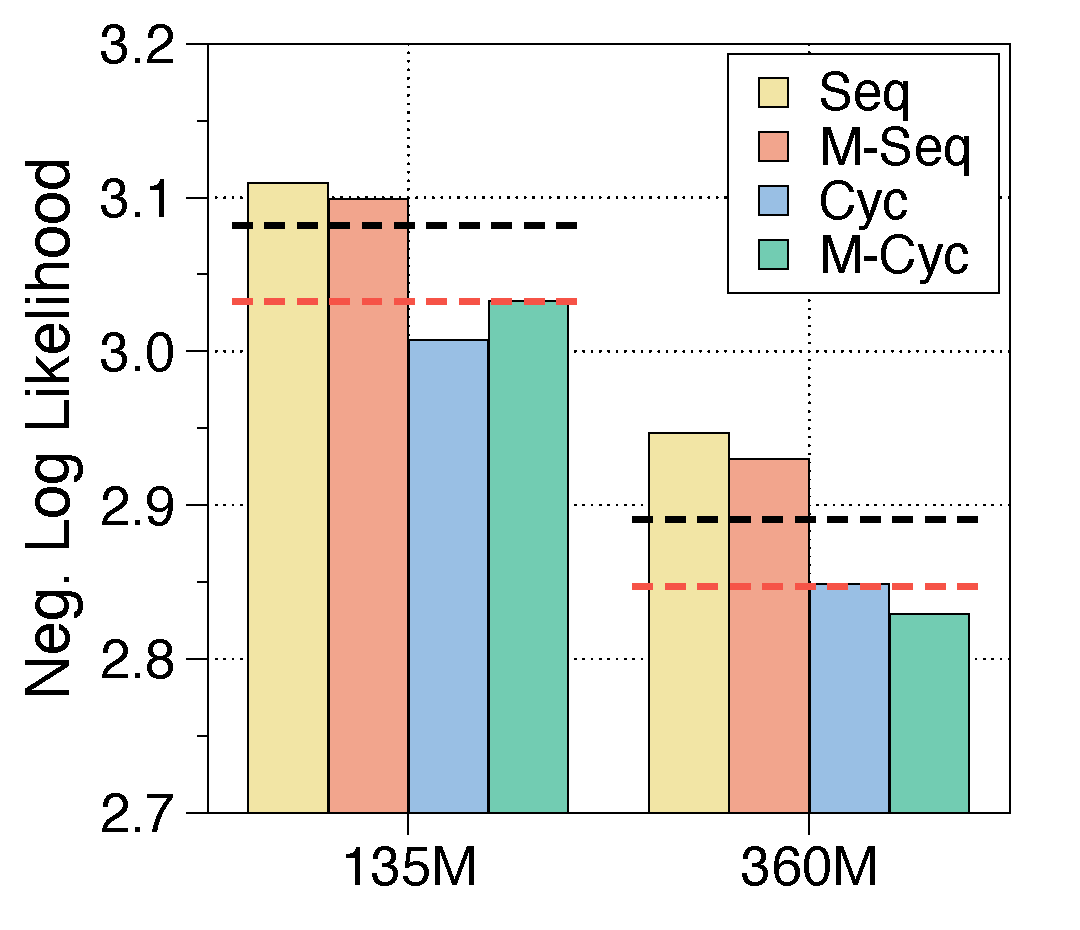
\includegraphics[width=\textwidth]{figs/revisit_sharing/revisit_sharing_rec2.pdf}
        \subcaption{Recursion of two\,($N_R$ = 2)}
        \label{fig:revisit_sharing_rec2_app}
    \end{subfigure}
    \hspace{10pt}
    \centering
    \begin{subfigure}[t]{0.35\textwidth}
    \captionsetup{justification=centering}
        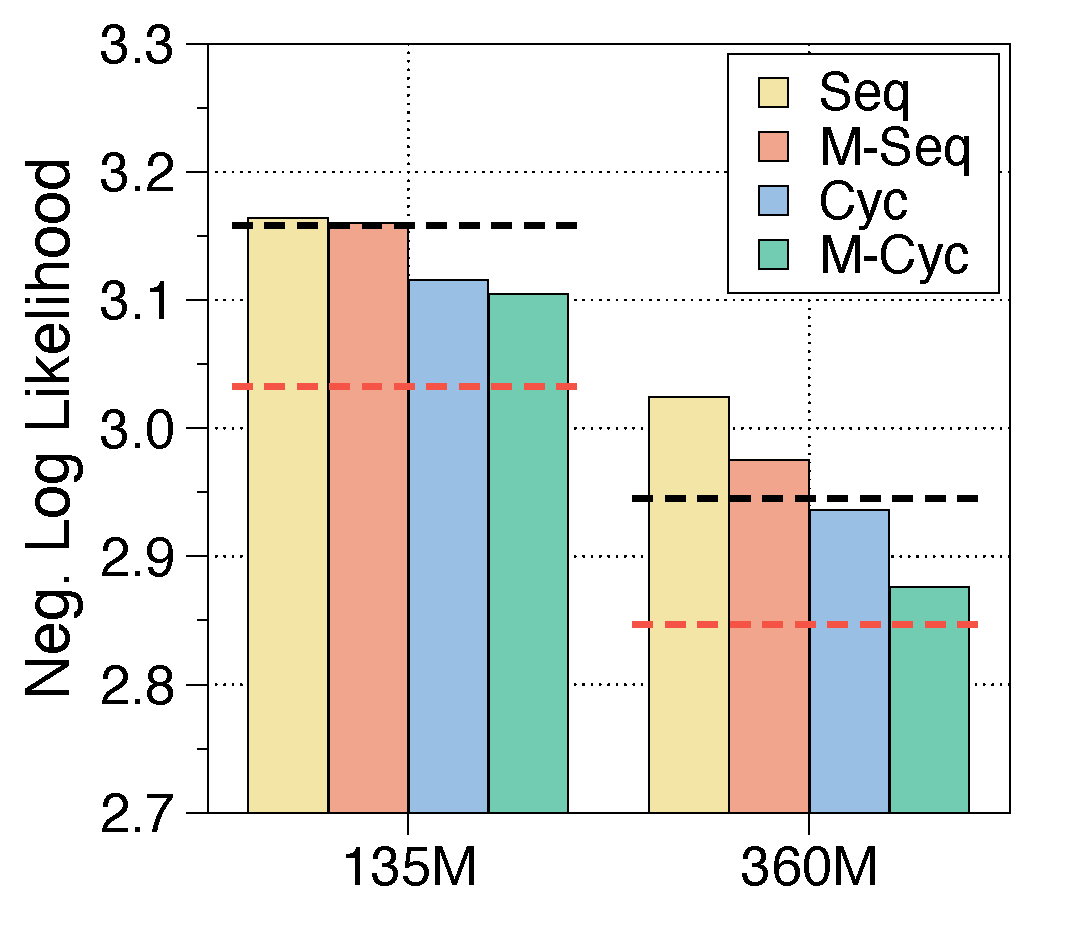
\includegraphics[width=\textwidth]{figs/revisit_sharing/revisit_sharing_rec3.pdf}
        \subcaption{Recursion of three\,($N_R$ = 3)}
        \label{fig:revisit_sharing_rec3_app}
    \end{subfigure}
    \caption{
    Validation negative log‑likelihood (lower is better) on \emph{FineWeb‑Edu} for four parameter‑sharing strategies.
    Bars are grouped by model capacity (135M vs.\ 360M parameters). 
    Middle‑Cycle consistently attains the lowest NLL, with its margin widening as either model size or depth increases.
    The horizontal dashed lines mark the \emph{untied} (non-sharing) baselines: the lower red line represents the full capacity model, while the upper black line represents a parameter-matched reduced model with a footprint equal to the unique trainable parameter sizes of the recursive model.
    }
    \label{fig:revisit_sharing_app}
\end{figure}
